%File: formatting-instructions-latex-2024.tex
%release 2024.0
\documentclass[letterpaper]{article} % DO NOT CHANGE THIS
\usepackage{aaai24}  % DO NOT CHANGE THIS
\usepackage{times}  % DO NOT CHANGE THIS
\usepackage{helvet}  % DO NOT CHANGE THIS
\usepackage{courier}  % DO NOT CHANGE THIS
\usepackage[hyphens]{url}  % DO NOT CHANGE THIS
\usepackage{graphicx} % DO NOT CHANGE THIS
\urlstyle{rm} % DO NOT CHANGE THIS
\def\UrlFont{\rm}  % DO NOT CHANGE THIS
\usepackage{natbib}  % DO NOT CHANGE THIS AND DO NOT ADD ANY OPTIONS TO IT
\usepackage{caption} % DO NOT CHANGE THIS AND DO NOT ADD ANY OPTIONS TO IT
\frenchspacing  % DO NOT CHANGE THIS
\setlength{\pdfpagewidth}{8.5in}  % DO NOT CHANGE THIS
\setlength{\pdfpageheight}{11in}  % DO NOT CHANGE THIS
%
% These are recommended to typeset algorithms but not required. See the subsubsection on algorithms. Remove them if you don't have algorithms in your paper.
\usepackage{dsfont}
\usepackage{amsmath}
\usepackage{amsfonts}
\usepackage{algorithm}
\usepackage{algorithmic}

\usepackage{makecell}
\usepackage{multirow}

%
% These are are recommended to typeset listings but not required. See the subsubsection on listing. Remove this block if you don't have listings in your paper.
\usepackage{newfloat}
\usepackage{listings}
\DeclareCaptionStyle{ruled}{labelfont=normalfont,labelsep=colon,strut=off} % DO NOT CHANGE THIS
\lstset{%
	basicstyle={\footnotesize\ttfamily},% footnotesize acceptable for monospace
	numbers=left,numberstyle=\footnotesize,xleftmargin=2em,% show line numbers, remove this entire line if you don't want the numbers.
	aboveskip=0pt,belowskip=0pt,%
	showstringspaces=false,tabsize=2,breaklines=true}
\floatstyle{ruled}
\newfloat{listing}{tb}{lst}{}
\floatname{listing}{Listing}
%
% Keep the \pdfinfo as shown here. There's no need
% for you to add the /Title and /Author tags.

% DISALLOWED PACKAGES
% \usepackage{authblk} -- This package is specifically forbidden
% \usepackage{balance} -- This package is specifically forbidden
% \usepackage{color (if used in text)
% \usepackage{CJK} -- This package is specifically forbidden
% \usepackage{float} -- This package is specifically forbidden
% \usepackage{flushend} -- This package is specifically forbidden
% \usepackage{fontenc} -- This package is specifically forbidden
% \usepackage{fullpage} -- This package is specifically forbidden
% \usepackage{geometry} -- This package is specifically forbidden
% \usepackage{grffile} -- This package is specifically forbidden
% \usepackage{hyperref} -- This package is specifically forbidden
% \usepackage{navigator} -- This package is specifically forbidden
% (or any other package that embeds links such as navigator or hyperref)
% \indentfirst} -- This package is specifically forbidden
% \layout} -- This package is specifically forbidden
% \multicol} -- This package is specifically forbidden
% \nameref} -- This package is specifically forbidden
% \usepackage{savetrees} -- This package is specifically forbidden
% \usepackage{setspace} -- This package is specifically forbidden
% \usepackage{stfloats} -- This package is specifically forbidden
% \usepackage{tabu} -- This package is specifically forbidden
% \usepackage{titlesec} -- This package is specifically forbidden
% \usepackage{tocbibind} -- This package is specifically forbidden
% \usepackage{ulem} -- This package is specifically forbidden
% \usepackage{wrapfig} -- This package is specifically forbidden
% DISALLOWED COMMANDS
% \nocopyright -- Your paper will not be published if you use this command
% \addtolength -- This command may not be used
% \balance -- This command may not be used
% \baselinestretch -- Your paper will not be published if you use this command
% \clearpage -- No page breaks of any kind may be used for the final version of your paper
% \columnsep -- This command may not be used
% % \newpage -- No page breaks of any kind may be used for the final version of your paper
% \pagebreak -- No page breaks of any kind may be used for the final version of your paperr
% \pagestyle -- This command may not be used
% \tiny -- This is not an acceptable font size.
% \vspace{- -- No negative value may be used in proximity of a caption, figure, table, section, subsection, subsubsection, or reference
% \vskip{- -- No negative value may be used to alter spacing above or below a caption, figure, table, section, subsection, subsubsection, or reference

\setcounter{secnumdepth}{0} %May be changed to 1 or 2 if section numbers are desired.

% The file aaai24.sty is the style file for AAAI Press
% proceedings, working notes, and technical reports.
%

% Title

% Your title must be in mixed case, not sentence case.
% That means all verbs (including short verbs like be, is, using,and go),
% nouns, adverbs, adjectives should be capitalized, including both words in hyphenated terms, while
% articles, conjunctions, and prepositions are lower case unless they
% directly follow a colon or long dash

\title{STAIR: Spatial-Temporal Reasoning with Auditable Intermediate Results for Video Question Answering}

\author{
    %Authors
    % All authors must be in the same font size and format.
    Yueqian Wang\textsuperscript{\rm 1},
    Yuxuan Wang\textsuperscript{\rm 2,3},
    Kai Chen\textsuperscript{\rm 4},
    Dongyan Zhao\textsuperscript{\rm 1,3}\thanks{Corresponding Author}
    % Francisco Cruz\equalcontrib,
    % Marc Pujol-Gonzalez\equalcontrib
}

\affiliations{
    % %Afiliations
    % \textsuperscript{\rm 1}Association for the Advancement of Artificial Intelligence\\
    % % If you have multiple authors and multiple affiliations
    % % use superscripts in text and roman font to identify them.
    % % For example,

    % % Sunil Issar\textsuperscript{\rm 2},
    % % J. Scott Penberthy\textsuperscript{\rm 3},
    % % George Ferguson\textsuperscript{\rm 4},
    % % Hans Guesgen\textsuperscript{\rm 5}
    % % Note that the comma should be placed after the superscript

    % 1900 Embarcadero Road, Suite 101\\
    % Palo Alto, California 94303-3310 USA\\
    % % email address must be in roman text type, not monospace or sans serif
    % proceedings-questions@aaai.org
% See more examples next

    % Affiliations
    \textsuperscript{\rm 1}Wangxuan Institute of Computer Technology, Peking University\\
    \textsuperscript{\rm 2}Beijing Institute for General Artificial Intelligence \\
    \textsuperscript{\rm 3}National Key Laboratory of General Artificial Intelligence\\
    \textsuperscript{\rm 4}School of Economics, Peking University\\
    wangyueqian@pku.edu.cn, wangyuxuan1@bigai.ai, chen.kai@pku.edu.cn, zhaodongyan@pku.edu.cn

}

%Example, Single Author, ->> remove \iffalse,\fi and place them surrounding AAAI title to use it
\iffalse
\title{My Publication Title --- Single Author}
\author {
    Author Name
}
\affiliations{
    Affiliation\\
    Affiliation Line 2\\
    name@example.com
}
\fi

\iffalse
%Example, Multiple Authors, ->> remove \iffalse,\fi and place them surrounding AAAI title to use it
\title{My Publication Title --- Multiple Authors}
\author {
    % Authors
    First Author Name\textsuperscript{\rm 1,\rm 2},
    Second Author Name\textsuperscript{\rm 2},
    Third Author Name\textsuperscript{\rm 1}
}
\affiliations {
    % Affiliations
    \textsuperscript{\rm 1}Affiliation 1\\
    \textsuperscript{\rm 2}Affiliation 2\\
    firstAuthor@affiliation1.com, secondAuthor@affilation2.com, thirdAuthor@affiliation1.com
}
\fi

\begin{document}

\maketitle

\begin{abstract}
Recently we have witnessed the rapid development of video question answering models. However, most models can only handle simple videos in terms of temporal reasoning, and their performance tends to drop when answering temporal-reasoning questions on long and informative videos.
To tackle this problem we propose \textbf{STAIR}, a \textbf{S}patial-\textbf{T}emporal Reasoning model with \textbf{A}uditable \textbf{I}ntermediate \textbf{R}esults for video question answering. STAIR is a neural module network, which contains a program generator to decompose a given question into a hierarchical combination of several sub-tasks, and a set of lightweight neural modules to complete each of these sub-tasks.
Though neural module networks are already widely studied on image-text tasks, applying them to videos is a non-trivial task, as reasoning on videos requires different abilities. In this paper, we define a set of basic video-text sub-tasks for video question answering and design a set of lightweight modules to complete them.
Different from most prior works, modules of STAIR return intermediate outputs specific to their intentions instead of always returning attention maps, which makes it easier to interpret and collaborate with pre-trained models. We also introduce intermediate supervision to make these intermediate outputs more accurate. We conduct extensive experiments on several video question answering datasets under various settings to show STAIR's performance, explainability, compatibility with pre-trained models, and applicability when program annotations are not available. Code: https://github.com/yellow-binary-tree/STAIR
\end{abstract}


\section{Introduction}
Video question answering (video QA) is a challenging task that lies between the field of Natural Language Processing and Computer Vision, which requires a joint understanding of text and video to give correct answers.
However, most approaches, including some recently proposed video-text large pre-trained models, only treat videos as animated images. They use black-box deep neural networks to learn mappings directly from inputs to outputs on factual questions like ``Who is driving a car?'', ignoring the biggest difference between videos and images: the existence of temporal information. As a result, their performance tends to drop when understanding long and informative videos and answering complicated temporal-reasoning questions, such as determining the order of two events, or identifying events in a given time period of the video, where small differences in temporal expressions can lead to different results.

In comparison, in image question answering, many neural-symbolic methods have been proposed to tackle with complicated spatial-reasoning problems. Neural Symbolic VQA \cite{yi2018neuralSymbolic} aims to parse a symbolic scene representation out of an image, and converts the question to a program that executes on the symbolic scene representation. Neural Symbolic Concept Learners \cite{Mao2019TheNC} also convert images to symbolic representations, but by learning vector representations for every visual concept.
However, though these neural symbolic methods can achieve very good results on synthetic images like CLEVR \cite{Johnson2016CLEVRAD} and Minecraft \cite{wu2017neural,yi2018neuralSymbolic}, they can not perform well on real-world images. One promising neural-symbolic approach is Neural Module Networks (NMNs) \cite{Andreas2015NeuralMN}. It first converts the question to a program composed of several functions using a program generator, and then executes the program by implementing each function with a neural network, which is also known as a ``module''. With the introduction of neural networks at execution, it works better on real-word image question answering like VQA \cite{Agrawal2015VQAVQ}, and can also provide clues about its reasoning process by checking the program and inspecting the output of its modules.

In this paper we apply the idea of NMN to video question answering and propose \textbf{STAIR}, a \textbf{S}patial-\textbf{T}emporal Reasoning model with \textbf{A}uditable \textbf{I}ntermediate \textbf{R}esults.

We define a set of basic video-text sub-tasks for video QA, such as localizing the time span of actions in the video, recognizing objects in a video clip, etc. We use a sequence-to-sequence program generator to decompose a question into its reasoning process, which is a hierarchical combination of several sub-tasks, and formalize this reasoning process into a formal-language program. Note that though the program generator requires question-program pairs to train, in practice we found that the program generator trained on AGQA2 \cite{GrundeMcLaughlin2022AGQA2} question-program pairs (which is publicly available) can generate plausible programs for questions from other datasets, so no further manual efforts are required to apply STAIR on video QA datasets without program annotations.

We also design a set of lightweight neural modules to complete each of these sub-tasks. These neural modules can be dynamically assembled into a neural module network according to the program. Then the neural module network takes video feature and text feature from a video encoder and a text encoder as input, and outputs a representation of the question after reasoning, which is then used by a classifier to generate the final answer. Different from most prior works of neural module networks, our neural modules return intermediate results specific to their intentions instead of always returning attention maps. Here we use the term ``auditable'' to describe that we can get the exact answer of each sub-task with no further actions required, which greatly increases the explainability of our method, and these intermediate results can also serve as prompts to improve the accuracy of pre-trained models.
We also introduce intermediate supervision to make the intermediate results more accurate by training neural modules with ground truth intermediate results.

We conduct experiments on the AGQA dataset \cite{GrundeMcLaughlin2021AGQA, GrundeMcLaughlin2022AGQA2}, a large-scale, real-world video question answering dataset with most questions of it require combinational temporal and logical reasoning to answer, for a detailed analysis of STAIR.
We also conduct experiments on STAR \cite{Wu2021STAR} and MSRVTT-QA \cite{Gao2018MotionAppearanceCN} to test the feasibility of STAIR on datasets without human annotations of programs. In summary, the contributions of this paper include:

\begin{itemize}
    \item We propose STAIR, a video question answering model based on neural module networks, which excels at solving questions that require combinational temporal and logical reasoning and is highly interpretable. We define sub-tasks for video QA, and design neural modules for the sub-tasks.
    \item We introduce intermediate supervision to make the intermediate results of the neural modules more accurate.
    \item We conduct extensive experiments on several video question answering tasks to demonstrate its performance, explainability, possibility to collaborate with pre-trained models, and applicability when program annotations are not available.
\end{itemize}


\section{Related Works}

\paragraph{Video Question Answering.}
Recent advances in video question answering methods can be roughly divided into four categories:
(1) \textbf{Attention based} methods \cite{Zhang2019OpenEndedLV,Li2019BeyondRP,Kumar2019LeveragingTA} that adopt spatial and/or temporal attention to fuse information from question and video;
(2) \textbf{Memory network based} methods \cite{Xu2017VideoQA,Gao2018MotionAppearanceCN,Fan2019HeterogeneousME,Kim2019ProgressiveAM} that use recurrent read and write operations to process video and question features;
(3) \textbf{Graph based} methods \cite{Jin2021AdaptiveSG,seo2021attend,Xiao2021VideoAC, Cherian2022251D, Park2021BridgeTA,Zhao2022Collaborative} that process videos as (usually object level) graphs and use graph neural networks to obtain informative video representations; and
(4) \textbf{Pre-trained models} \cite{Lei2021LessIM,Fu2021VIOLETE,Zellers2021MERLOTMN,Zellers2022MERLOTRN,Wang2023Vstar} that pre-train a model in self-supervised manner with a mass of video-text multi-modal data. Recently, many works also try to solve video QA in zero-shot settings using large pre-trained transformer-based models \cite{Alayrac2022FlamingoAV, Li2023VideoChatCV, Zhang2023VideoLLaMAAI, Lyu2023MacawLLMML}. Though many works have reported good video understanding and response generation abilities of their models, these models require massive computing resources to pre-train, and their training videos/questions are relatively simple in terms of temporal reasoning, which means that these models are not robust at understanding and reasoning temporal information of videos.

Since there is usually redundant information in the video, Some works \cite{Kim2020ModalitySA, Gao2022MISTMI, Li2022InvariantGF} also study helping the model focus on key information by selecting video clips relevant to the question.

Though the above-mentioned methods have achieved outstanding performance, for most of these methods their performance tends to drop when evaluating on questions that require complicated logical reasoning or counterfactual questions and are difficult to interpret. To tackle these problems, some works use neural symbolic approach \cite{yi2019clevrer} \cite{Qian2022DynamicSM} or construct physics models \cite{Ding2021DynamicVR,chen2021grounding}.

\paragraph{Neural Module Networks.}
Neural Module Networks (NMN) have been widely used in image question answering \cite{Andreas2015NeuralMN,Hu2017LearningTR,Johnson2017InferringAE,Mascharka2018TransparencyBD,Hu2018ExplainableNC}. These methods explicitly break down questions into several sub-tasks and solve each of them with a specifically-designed neural network (module). Attention maps or image representations are used to pass information among modules. Neural Module Networks are generally more interpretable, and excel at tasks that require compositional spatial reasoning such as SHAPES \cite{Andreas2015NeuralMN} and CLEVR \cite{Johnson2016CLEVRAD}.
A more advanced NMN for image-text tasks is the recently-proposed Visual Programming \cite{Gupta2023VisualProgramming}.
Taking advantage of several off-the-shelf models such as CLIP \cite{Radford2021LearningTV}, GPT-3 \cite{Brown2020LanguageMA} and Stable Diffusion \cite{rombach2021highresolution}, Visual Programming is capable of performing image QA, object tagging, and natural language image editing without further training.

Contrary to the intense research efforts of NMNs on image QA, there are significantly fewer works that focus on video QA \cite{Le2022VGNMNVN, Qian2022DynamicSM}. Though sharing the same motivation, it is non-trivial to define the sub-tasks and design their corresponding modules for video modality, which is one of the main contributions of our work. The work most similar to ours is DSTN \cite{Qian2022DynamicSM}, which also uses neural module network for video QA. But our work is significantly different from theirs in better performance, better explainability, the usage of intermediate supervision, the ability to collaborate with pre-trained models, and verifying its applicability when program annotations are not available.

\section{Methodology}
\begin{figure*}[t]
    \centering
    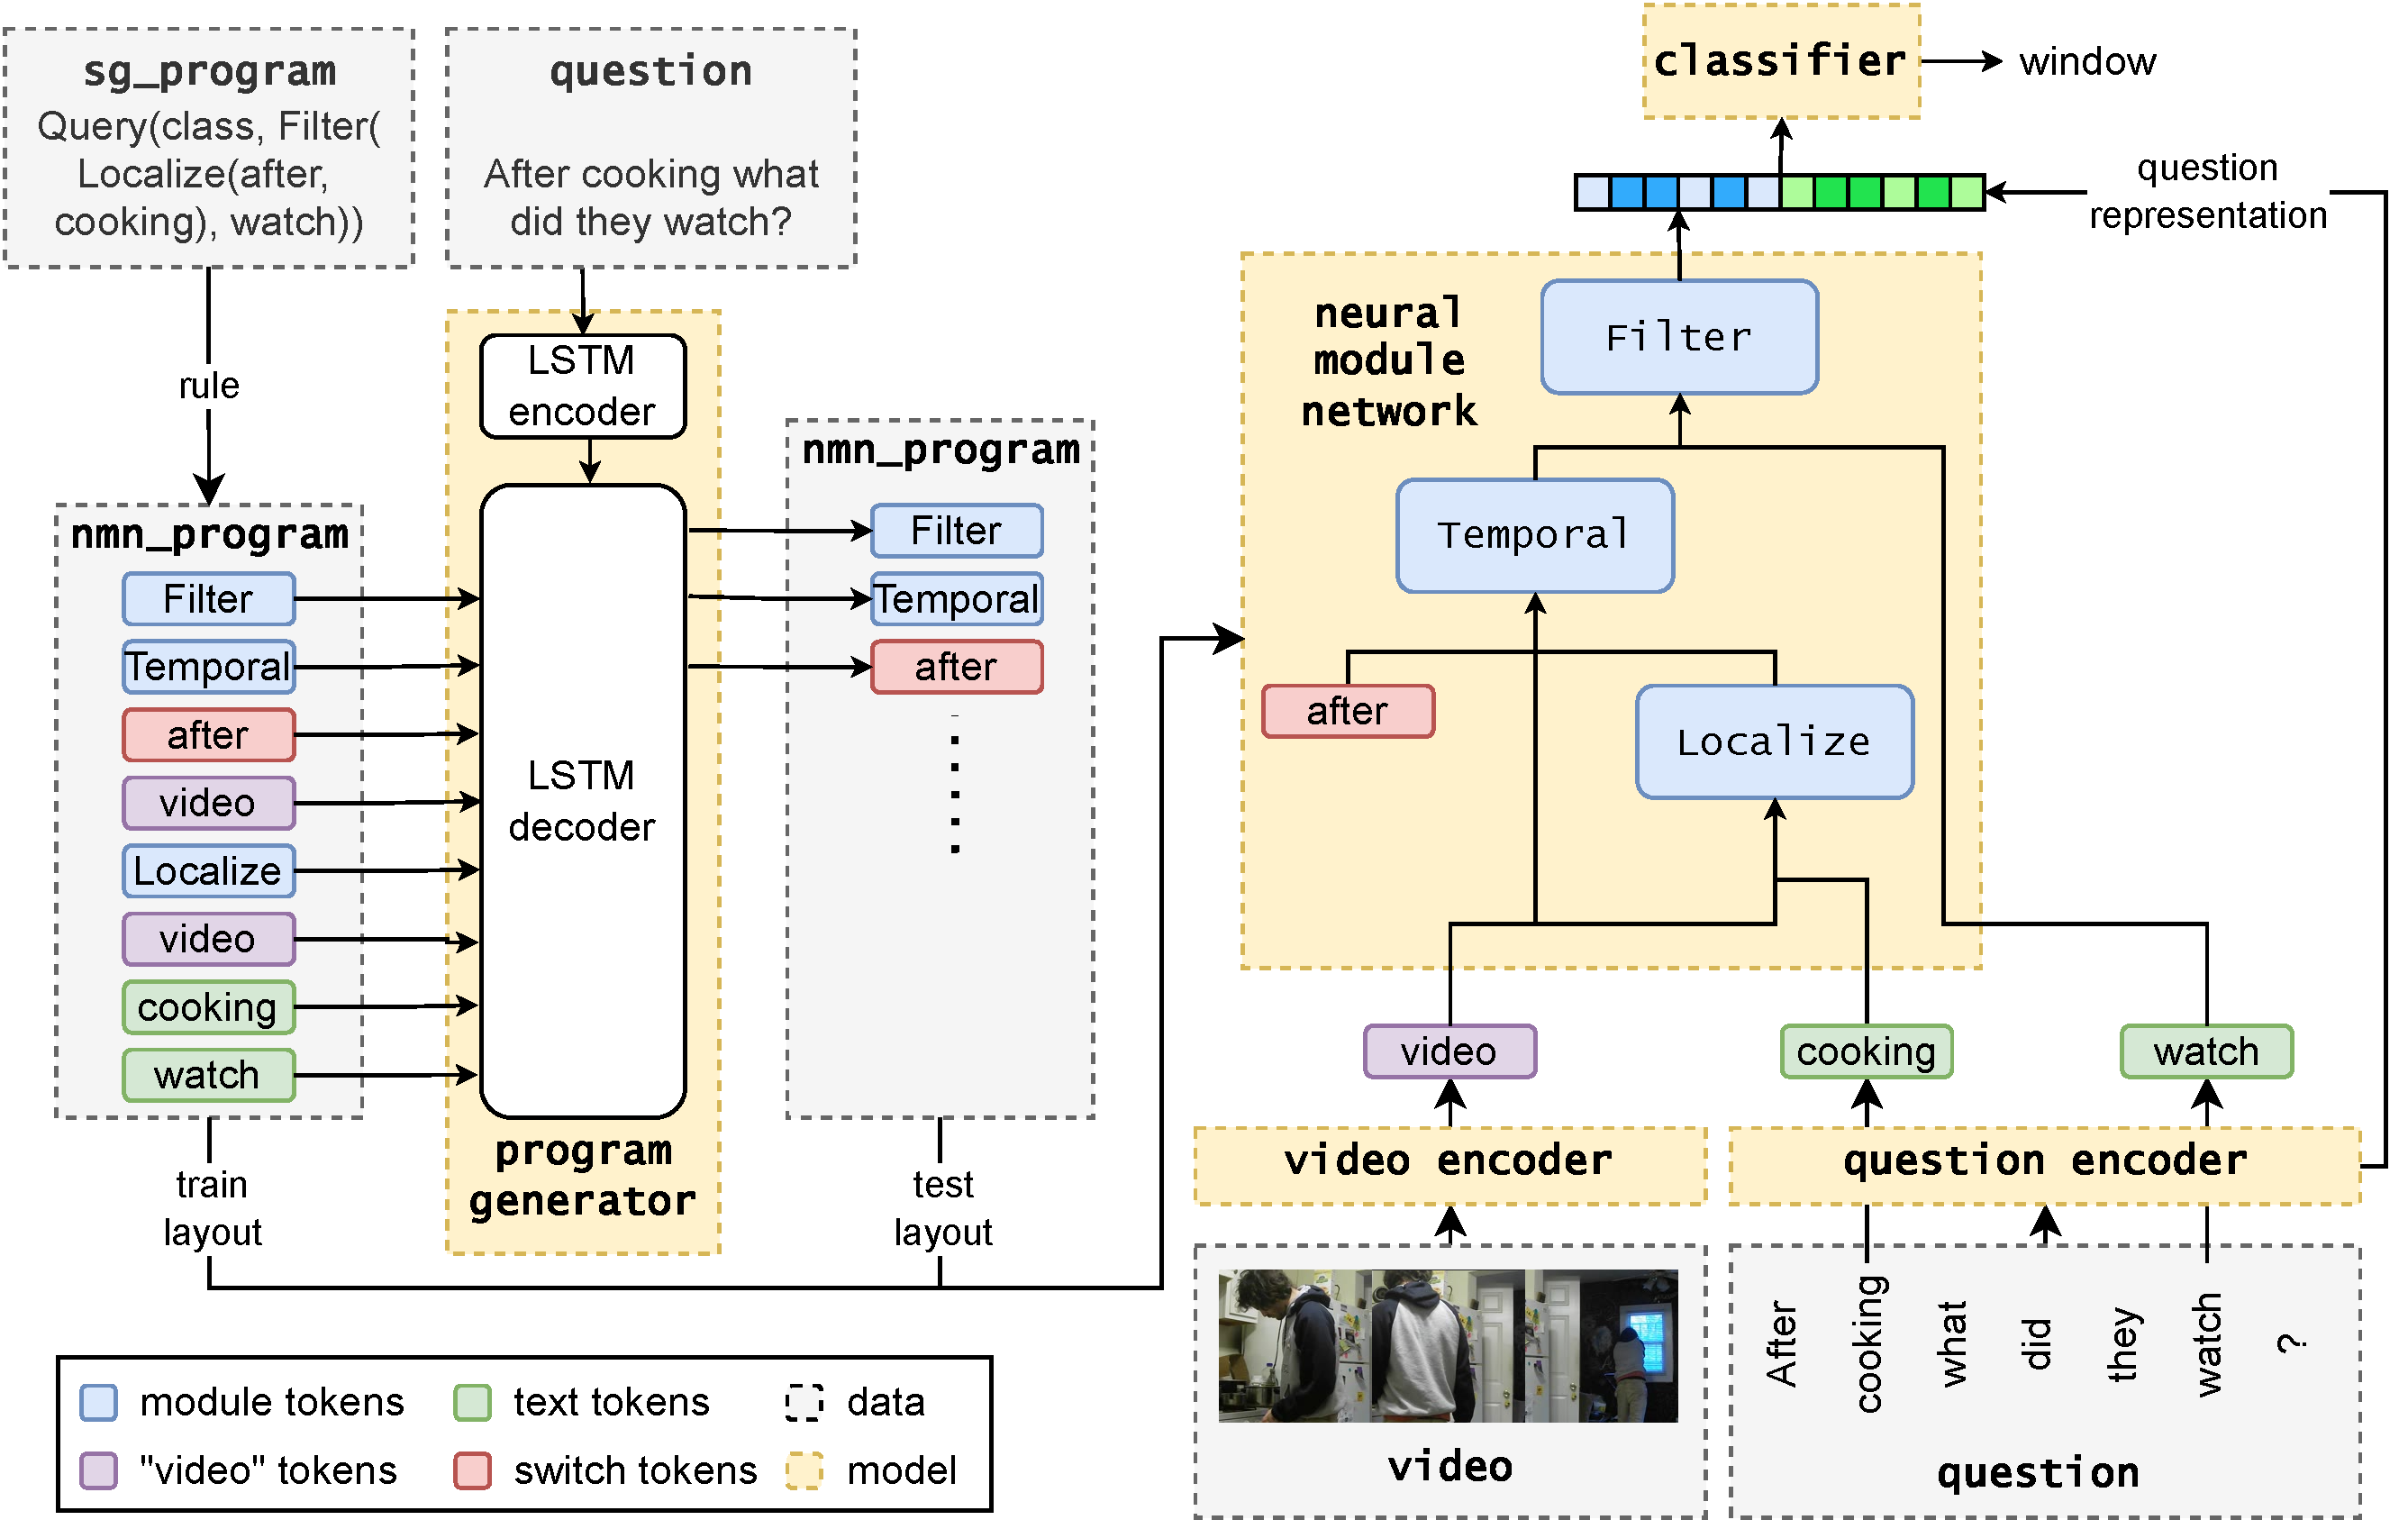
\includegraphics[width=0.9\textwidth]{plt/overview.png}
    \caption{Overview of STAIR.}
    \label{fig:overview}
\end{figure*}

In this section, we describe the details of STAIR. STAIR takes as input a video feature $x_v \in \mathbb{R}^{T \times hid_V}$ with $T$ frames encoded by a pre-trained visual feature extractor and a question $x_q$ with $L$ words, and selects an answer $a$ from a fixed set of all possible answers $\mathcal{A}$. STAIR consists of the following components:
(1) a bi-directional LSTM \textbf{video encoder} ${ENC}_{vid}$ which models the temporal relationship of the video feature and transforms it into the common hidden space $v = {ENC}_{vid}(x_v), v \in \mathbb{R}^{T \times H}$; (2) a bi-directional LSTM \textbf{text encoder} ${ENC}_{txt}$ which extracts the sentence-level and token-level question feature as $(q, t)={ENC}_{txt}(x_q), q \in \mathbb{R}^H, t \in \mathbb{R}^{L \times H}$; (3) \textbf{a collection of neural modules} $\{f_m\}$, each of which has a set of associated parameters $\theta_m$, performs a specific sub-task, and can be combined into a neural module network; and (4) a two-layer \textbf{classifier} $\phi(\cdot)$ that predicts the final answer. Besides, a \textbf{program generator} $p = gen(x_q)$ is trained individually to predict the program that determines the layout of the modules given a question $x_q$. The overview of the model is shown in Figure \ref{fig:overview}.

\subsection{Neural Modules}
As mentioned above, our solving process of the questions can be decomposed into several sub-tasks. For example, to answer the question \textit{"After cooking some food what did they watch?"}, there are 3 sub-tasks to solve: first localize the clips among the entire video when the people are cooking, then navigate to clips that happen after the cooking clips, and finally focus on these clips to find out the object that the people are watching.

Our STAIR contains 16 neural modules implementing different sub-tasks. All of these modules are implemented by simple neural networks such as several linear layers or convolutional layers. Their inputs, outputs, and intended functions are very diverse, including \texttt{Filter} module that finds objects or actions from a given video clip, \texttt{Exists} module that determines whether an object exists in the results of \texttt{Filter}, \texttt{Localize} module that finds in which frames an action happens, to name a few. The intentions and implementation details of all modules are listed in the Appendix. Different from most of the previous works of neural module networks, the inputs and outputs of our modules are not always the same (e.g., attention maps on images/videos), but are determined by the intentions of each module. Take the module \texttt{Filter(video,objects)} as an example, it intends to find all objects that appear in the video. Instead of returning an attention map showing when the objects occur, in our implementation it must return a feature vector from which we can predict the names of all objects in the video. This design leads to significantly better explainability and reliability, as we can know the exact objects it returns by only inspecting the output.

\subsection{Programs and the Program Generator}
The design of the program is inspired by the AGQA dataset. In AGQA, each question is labeled with a program consisting of nested functions indicating the sub-tasks of this question, and each video is tagged with a video scene graph from Charades and Action Genome \cite{sigurdsson2016hollywood,Ji2019ActionGA}. The answer can be acquired by executing the program on the scene graph. We use a rule-based approach to convert the labeled program to a sequence of program tokens, which is the Reverse Polish Notation of the tree-structured layout of our modules. \footnote{For details of this rule-based approach please refer to our code.} To avoid confusion hereafter we refer to the program before and after conversion as \texttt{sg\_program} and \texttt{nmn\_program}. Note that though \texttt{nmn\_program} is designed according to \texttt{sg\_program} in AGQA, it also works on other video question answering tasks as shown in Section \ref{sec:other_task}.

Program tokens in \texttt{nmn\_program} can be categorized into 4 types: (1) \textbf{module tokens} which corresponds to a neural module, e.g., \texttt{Filter}, \texttt{Localize}; (2) \textbf{the ``video'' token} that represents the video feature $v$; (3) \textbf{text tokens} which corresponds to a text span in the question $x_q$, e.g., ``watch'', ``cooking some food''; and (4) \textbf{switch tokens} which are keywords switches between the branches in a module, e.g., ``max'', ``after'', ``fwd''(``forward'').

As \texttt{nmn\_program}s are not provided during inference, we need to train a program generator to learn the mappings from questions to \texttt{nmn\_program}s. We tried fine-tuning a FLAN-T5-large \cite{wei2021finetunedLM}, but this problem is easy as a simple bi-directional LSTM encoder-decoder model with attention can predict exactly the right \texttt{nmn\_program} for more than 98\% of the questions in AGQA, so we decide to use the light-weight LSTM here.

\begin{figure}[t]
    \centering
    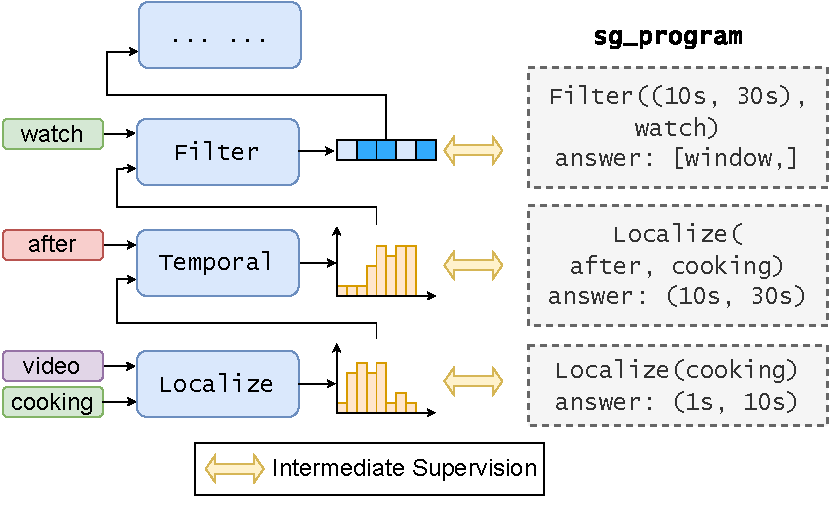
\includegraphics[width=0.5\textwidth]{plt/intermediate_supervision.png}
    \caption{A Diagram of Intermediate Supervision.}
    \label{fig:intermediate_supervision}
\end{figure}

\subsection{Intermediate Supervision}
Previous works mentioned that sometimes modules in the neural module networks do not behave as we expected and thus can't provide meaningful intermediate outputs for us to understand its reasoning steps despite predicting the final answer correctly \cite{Hu2017LearningTR}. To mitigate this problem, we use \textbf{intermediate supervision} to induce supervision to intermediate modules. An example of intermediate supervision is shown in Figure \ref{fig:intermediate_supervision}.
Given that \texttt{nmn\_program} is obtained by converting \texttt{sg\_program} using a rule-based approach, we can record the correspondence between functions in \texttt{sg\_program} and modules in \texttt{nmn\_program}. Then we execute \texttt{sg\_program} on the video scene graph and take the return value of functions as ground truth answers of corresponding modules. \footnote{As the authors of AGQA and Action Genome do not release their code of acquiring answers via scene graphs, we have to implement these functions by ourselves. For about 5\% of all training examples, our implementation can't return the correct final answer given \texttt{sg\_program} and scene graph of the corresponding video, so we don't use intermediate supervision on them.} We use intermediate supervision for all but the first module in \texttt{nmn\_program} (i.e., the root module in the tree structure), as the first module is already directly supervised by the answer. Note that intermediate supervision does not always improve the model's performance, as its main purpose is to make the outputs of intermediate modules more accurate.
Depending on the data type, we use different criteria to calculate the intermediate supervision loss $\mathcal{L}^{IS}$ between the gold answer and module prediction, which is elaborated in the Appendix.

\subsection{Training Procedures}
The program generator is trained individually, and the main model, including video encoder, text encoder, neural modules, and classifier are trained in an end-to-end manner.

Generating \texttt{nmn\_program} is considered as a sequence-to-sequence task. A model $gen(\cdot)$ takes question $x_q$ as input and generate \texttt{nmn\_program} $\hat{p}$ in an auto-regressive manner:

\begin{equation}
logP(\hat{p}|x_q) = \sum_t log(\hat{p_t} | x_q, \hat{p}_{<t})
\end{equation}

and the loss $\mathcal{L}^{GEN}$ is calculated using the negative log likelihood of ground truth \texttt{nmn\_program} $p$:

\begin{equation}
\mathcal{L}^{GEN}=-\sum_t log(p_t| x_q, p_{<t})
\end{equation}

When training the main model, the ground truth \texttt{nmn\_program} of train and valid set, or the \texttt{nmn\_program} generated by the program generator of test set is used to assemble the neural modules ${f_m}$ into a tree-structured neural module network. The classifier loss $\mathcal{L}^{CLS}$ is calculated using the ground truth answer $a$ and the predicted logits $\hat{a}$ over all candidate answers produced by the classifier as:

\begin{equation}
\mathcal{L}^{CLS}=l_{ce}(\hat{a}, a)
\end{equation}

The total loss of the main model is $\mathcal{L}=\mathcal{L}^{CLS}+\eta \mathcal{L}^{IS}$, where $\eta$ is a hyper-parameter balancing the classifier loss and the intermediate supervision loss.


\section{Experiments}
We evaluate STAIR mainly on AGQA balanced dataset \cite{GrundeMcLaughlin2021AGQA}, as it is a large-scale, real-world video QA dataset with most questions in it requiring comprehensive temporal reasoning to answer. AGQA balanced dataset contains 3.9M question-answer pairs with 9.6K videos. Each question is associated with a program that describes the reasoning steps to answer the questions. Videos in AGQA are from Charades \cite{sigurdsson2016hollywood}, a diverse human action recognition dataset collected by hundreds of people in their own homes. Each video is annotated with a video scene graph containing spatial and temporal information about actions and objects from Action Genome \cite{Ji2019ActionGA}. AGQA is very challenging, as even state-of-the-art deep learning models perform much worse than humans. We also evaluate on AGQA2 balanced dataset \cite{GrundeMcLaughlin2022AGQA2} which contains 2.27M question-answer pairs selected with a stricter balancing procedure and is even more challenging than AGQA. Following \cite{Le2020HierarchicalCR}, we leave 10\% of the train set out as valid set, and require videos in train/valid set to be different.

\subsection{Model Implementations}
\paragraph{Implementation.} We used two different video features in our experiments. One is the standard video features provided by the AGQA dataset, including appearance features $x_v^a \in \mathbb{R}^{8 \times 16 \times 2048}$ extracted from ResNet-101 pool5 layer\cite{He2015DeepRL}, and motion features $x_v^m \in \mathbb{R}^{8 \times 2048}$ extracted from ResNeXt-101\cite{Xie2016AggregatedRT}. We use mean pooling on the second dimension of $x_v^a$ and concatenate it with $x_v^m$ to obtain the final video feature $x_v \in \mathbb{R}^{8 \times 4096}$. We name this video feature ``RX''. However, as the official RX feature only has 8 frames on temporal dimension which is insufficient for complicated temporal reasoning, we also extract a video feature ourselves. We sample frames from videos with a frame rate of 24 fps, and use an I3D model pre-trained on Kinetics \cite{Carreira2017QuoVA} to extract a 1024-d feature for every consecutive 16 frames. We clip the temporal dimension length to 64, so the final video feature is $x_v \in \mathbb{R}^{T \times 1024}, T\leq64$. We name this video feature ``I3D''.

STAIR is trained with batch size 32, initial learning rate 2e-4 and decays linearly to 2e-5 in 200k steps. $\eta$ is set as 1. STAIR is trained on a Nvidia A100 GPU, and it takes about 2 epochs (30 hours) on average for a single run.

\paragraph{Baselines.} We compare \textbf{STAIR} with and without intermediate supervision (\textbf{-IS}) with several baselines. We compare with 3 representative video QA models: \textbf{HME} \cite{Fan2019HeterogeneousME} is a memory-network-based model to encode video and text features; \textbf{HCRN} \cite{Le2020HierarchicalCR} uses conditional relational networks to build a hierarchical structure that learns video representation on both clip level and video level; \textbf{PSAC} \cite{Li2019BeyondRP} uses both video and question positional self-attention instead of RNNs to model dependencies of questions and temporal relationships of videos.
To compare with models that explicitly model the multi-step reasoning process, we also compare with \textbf{DSTN} \cite{Qian2022DynamicSM}, a neural module   network concurrent to our work, and \textbf{MAC} \cite{hudson2018compositional} which performs iterative attention-based reasoning with a recurrent ``Memory, Attention and Composition'' cell. We make minor modifications on the attention of MAC to attend to 2-D $(T \times dim_V)$ temporal features instead of 3-D $(H \times W \times dim_V)$ spatial features.

\begin{table}[t]
    \centering
    \setlength{\abovecaptionskip}{5pt}
    \resizebox{0.99\columnwidth}{!}{
    \begin{tabular}{cc|ccc|c}
            \hline
            \textbf{Methods} & \textbf{Video} & \textbf{Binary} & \textbf{Open} & \textbf{Overall} & \textbf{\#Prm} \\
            \hline
            % RX feature
            PSAC \dag & RX & 53.56 & 32.19 & 42.44 & 39M \\
            HME \dag & RX & 57.21 & 36.57 & 46.47 & 42M \\
            HCRN \dag & RX & 56.01 & 40.27 & 47.82 & 41M \\
            MAC & RX & 57.74 & 41.24 & 49.15 & 16M \\
            DSTN-E2E \dag & RX & 57.38 & 42.43 & 49.60 & 36M \\
            STAIR & RX & 59.07 & \textbf{43.08} & 50.75 & 21M \\
            STAIR-IS & RX & \textbf{60.15} & 42.84 & \textbf{51.14} & 21M \\
            \hline
            % I3D feature
            MAC & I3D & 58.19 & 46.84 & 52.28 & 10M \\
            STAIR & I3D & 60.18 & 47.24 & 53.45 & 14M \\
            STAIR-IS & I3D & \textbf{62.37} & \textbf{48.32} & \textbf{55.06} & 15M \\
            \hline
    \end{tabular}}
    \caption{Results of AGQA. \dag: Results from \cite{Qian2022DynamicSM}. \#Prm denotes number of parameters. \#Prm of MAC varies slightly with its number of steps, here we show \#Prm of a 12-step model.}
    \label{tab:agqa1}
\end{table}


\begin{table}[t]
    \centering
    \setlength{\abovecaptionskip}{5pt}
    \setlength{\tabcolsep}{4pt}
    \begin{tabular}{cc|ccc}
    \hline
    \textbf{Methods} & \textbf{Video} & \textbf{Binary} & \textbf{Open} & \textbf{Overall} \\
    \hline
    % I3D feature
    MAC & I3D & 54.72 & 44.96 & 49.67 \\
    STAIR & I3D & \textbf{57.13} & \textbf{47.07} & \textbf{52.06} \\
    STAIR-IS & I3D & 56.48 & 46.41 & 51.41 \\
    \hline
    \end{tabular}
    \caption{Results of AGQA2.}
    \label{tab:agqa2}
\end{table}

\begin{table}[t]
    \centering
    \setlength{\abovecaptionskip}{5pt}
    \setlength{\tabcolsep}{4pt}
    \begin{tabular}{c|ccc}
    \hline
    \multirow{2}{*}{\textbf{Methods}} & \textbf{Filter} & \textbf{Localize} & \textbf{Temporal} \\
     & (R@1/5) & (IoU) & (IoU) \\
    \hline
    Baseline & 0.11/0.43 & 0.16 & 0.13 \\
    STAIR & 0.12/0.30 & 0.19 & 0.35 \\
    STAIR-IS & \textbf{0.25/0.50} & \textbf{0.23} & \textbf{0.40} \\
    \hline
    \end{tabular}
    \caption{Performances of Filter, Localize and Temopral modules.}
    \label{tab:interpret}
\end{table}

\subsection{Model Performance}
Table \ref{tab:agqa1} shows the accuracy of all models on binary, open-ended and all questions of AGQA. STAIR outperforms all other baselines when using the same video feature, demonstrating the effectiveness of our approach. All models using the I3D video feature outperform their counterparts that use the RX feature, which shows the higher quality of I3D features. We also find that intermediate supervision does not always improve the performance of STAIR, probably due to the coordination problems among the losses of multi-task learning. However intermediate supervision does improve the model's explainability by making the output of intermediate results more accurate, which is shown in the next subsection. We also compare STAIR with the strongest baseline MAC using the I3D video feature on AGQA2, and the results are shown in Table \ref{tab:agqa2}.

\subsection{Evaluation and Visualization of Modules' Intermediate Output}
As our STAIR is based on neural module networks, it enjoys good interpretability while performing well.
To demonstrate the interpretability of STAIR, we evaluate the intermediate results of \texttt{Filter}, \texttt{Localize} and \texttt{Temporal} modules, as these modules occurs at high frequency, and the outputs of them are intuitive and easy to inspect.

\texttt{Filter} module is designed to find objects and actions in the video or related to a given verb. To check the correctness of the output from \texttt{Filter} module, we use Recall@$N$ in a retrieval task as the evaluation metric. We calculate a candidate representation for each of the 214 candidate answers, and use cosine similarity between the output of \texttt{Filter} module and candidate representations to select a list of $N$ most likely predictions. If one of the predicted items occurs in the list of ground truth action(s)/object(s), we count it as a successful retrieval. We use the most frequently occurring $N$ actions/objects as baseline results.

\texttt{Localize} module is designed to find when an action happens in a video. We use $IoU_{att}$ as the evaluation metric. Given the predicted and ground truth attention scores $att_{p}, att_{g} \in \mathbb{R}^T$, the metric $IoU_att$ is calculated as $IoU_{att}=sum(min(att_{p}, att_{g})) / sum(max(att_{p}, att_{g}))$, where $max$ and $min$ are element-wise operations. We use uniform distribution as baseline attention scores: $att_{b} \sim \mathbf{U}(0,1) \times T$.

\texttt{Temporal} module is designed to transform the attention scores according to the switch keyword $s$. We use the same metric $IoU_{att}$ to evaluate the attention scores output $att_{out}$. Inspired by \cite{Qian2022DynamicSM}, we randomly sample two frames as the start and end frames as baseline results. Specially, the start frame is always the first frame when $s=$ `before', and the end frame is always the last frame when $s=$ `after'.

Table \ref{tab:interpret} shows the results. STAIR performs baseline on most metrics except R@5 of \texttt{Filter} module, which indicates that STAIR is capable of providing meaningful intermediate results, and training with intermediate supervision can make the intermediate results more accurate.


We also visualize the reasoning process of STAIR on some real examples in the test set in the Appendix.

\begin{table*}[t]
    \setlength{\abovecaptionskip}{5pt}
    \centering
    \begin{tabular}{c|ccc|ccc|c}
        \hline
        \multirow{2}{*}{\textbf{Methods}} & \multicolumn{3}{c|}{\textit{AGQA}} & \multicolumn{3}{c|}{\textit{AGQA2}} & \multirow{2}{*}{\textbf{\#Params}} \\
        & \textbf{Binary} & \textbf{Open} & \textbf{Overall} & \textbf{Binary} & \textbf{Open} & \textbf{Overall} & \\
        \hline
        STAIR & 60.18 & 47.24 & 53.45 & 57.13 & 47.07 & 52.06 & 14.97M \\
        STAIR-IS & 62.37 & 48.32 & 55.06 & 56.48 & 46.41 & 51.41 & 15.11M \\
        GPT-2 & 63.94 & 50.88 & 57.14 & 58.10 & 47.90 & 52.96 & 127M \\
        Violet & 60.87 & \textbf{52.88} & 56.72 & 50.28 & \textbf{49.93} & 50.11 & 160M \\
        \makecell[c]{GPT-2+ \\ STAIR-IS} & \textbf{64.26} & 50.97 & \textbf{57.34} & \textbf{60.46} & 49.86 & \textbf{55.13} & \makecell[c]{127M+ \\ 15.11M} \\
        \hline
    \end{tabular}
    \caption{Results of AGQA and AGQA2, comparing with pre-trained models.}
    \label{tab:pretrain}
\end{table*}

\begin{table}[t]
    \centering
    % \setlength{\abovecaptionskip}{5pt}
    % \setlength{\tabcolsep}{4pt}
    \begin{tabular}{c|c}
        \hline
        \textbf{Methods} & \textbf{Overall} \\
        \hline
        Video-ChatGPT & 35.09 (0.76) \\
        + STAIR-IS & \textbf{40.43} (0.89) \\
        \hline
    \end{tabular}
    \caption{Results of Video-ChatGPT on AGQA2.}
    \label{tab:zs_agqa2}
\end{table}


\subsection{Compatibility with Pre-trained Models}
Pre-trained models, including text-only ones and multi-modal ones, have achieved state-of-the-art performance on many question answering tasks. Here we first compare STAIR with a single-modal pre-trained model \textbf{GPT-2} \cite{Radford2019LanguageMA}, and a video-text pre-trained model \textbf{Violet} \cite{Fu2021VIOLETE}.
For GPT-2, we prepend I3D video features to questions and assign different token type embeddings following \cite{Li2020BridgingTA}.
For Violet, we sampled $T=10$ video frames, resize them into $224 \times 224$, and split them into patches with $W \times H = 32 \times 32$. Though we can't use the pre-trained temporal position embedding as our $T=10$ is larger than $T=4$ in the pre-training stage and $T=5$ for downstream tasks in the original paper, we find that this gives better results. Table \ref{tab:pretrain} shows that on AGQA STAIR still underperforms GPT-2 and Violet, probably due to significantly fewer parameters and the absence of pre-training.
However, the performance gap between STAIR and the pre-trained models on AGQA2 is smaller, probably due to the language bias being further reduced and it's harder for pre-trained models to find textual clues to solve the questions.

To combine STAIR with pre-trained models, we use a straightforward method: we modify the questions to add the intermediate results of our neural modules to the input of pre-trained models as prompts. We get the top 1 candidate result for every \texttt{Filter} module in STAIR-IS using methods described in intermediate output subsection, and concatenate it with its keyword inputs. As \texttt{Filter} modules with lower levels have higher accuracy, we sort all \texttt{Filter} modules in ascending order of level and take only the first $\mathbf{P}$ modules into account, where $\mathbf{P}$ is selected in \{1,3,5\} by valid set performance. Take the following question as an example: \textit{What did they take while sitting in the thing they went above?}. To answer this question, the corresponding \texttt{nmn\_program} contains one \texttt{Filter} module with parameter $(video, above)$ and returns the result ``bag". So the modified question becomes: \textit{above bag. What did they take while sitting in the thing they went above?}. This can reduce the difficulty of questions by providing answers to some sub-tasks so it requires fewer steps to answer them.
We use this method on the best-performing GPT-2 and denote it as \textbf{GPT-2+STAIR-IS}. Experiments show that with the help of these intermediate outputs, the performance of GPT-2 is further improved. It is also an evidence of the usefulness of the intermediate results.

Given the recent rapid development of multi-modal large pre-trained models, we also report the results of zero-shot \textbf{Video-ChatGPT} \cite{Maaz2023VideoChatGPTTD}, a video-text pre-trained model which is claimed to be optimized for temporal understanding in videos, and \textbf{Video-ChatGPT + STAIR-IS} in Table \ref{tab:zs_agqa2}. Following \cite{Maaz2023VideoChatGPTTD}, Video-ChatGPT is not fine-tuned, and we benchmark its performance on AGQA2 with the evaluation pipeline using GPT-3.5. As it is unfeasible to test on the entire test set of AGQA2 with 660K questions, we randomly sample 1\% (6.6K questions), repeat the experiment for 3 times, and report the average accuracy and standard deviation.

\begin{table}[t]
\setlength{\abovecaptionskip}{5pt}
\setlength{\tabcolsep}{3pt}
    \centering
    % \resizebox{0.8\columnwidth}{!}{
    \begin{tabular}{c|cccc}
        \hline
        \textbf{Methods} & \textbf{Int.} & \textbf{Seq.} & \textbf{Pre.} & \textbf{Fea.} \\
        \hline
        CNN-BERT \dag & 33.59 & 37.16 & 30.95 & 30.84 \\
        L-GCN \dag & 39.01 & 37.97 & 28.81 & 26.98 \\
        HCRN \dag & \textbf{39.10} & 38.17 & 28.75 & 27.27 \\
        STAIR & 33.20 & \textbf{39.16} & \textbf{38.41} & \textbf{31.30} \\
        \hline
        ClipBERT \dag & 39.81 & 43.59 & 32.34 & 31.42 \\
        \hline
    \end{tabular} % }
    \caption{Accuracy on STAR test set, categorized by question type. \dag: Results from \cite{Wu2021STAR}}
    \label{tab:star}
\end{table}

\begin{table}[t]
    \centering
    % \resizebox{0.95\columnwidth}{!}{
    \begin{tabular}{c|c}
        \hline
        \textbf{Methods} & \textbf{MSRVTT-QA} \\
        \hline
        Co-Memory \cite{Gao2018MotionAppearanceCN} & 32.0 \\
        HME \cite{Fan2019HeterogeneousME} & 33.0 \\
        HCRN \cite{Le2020HierarchicalCR} & \textbf{35.6} \\
        STAIR & 34.8 \\
        \hline
        ClipBERT \cite{Lei2021LessIM} & 37.4 \\
        \hline
    \end{tabular} % }
    \caption{Accuracy on MSRVTT-QA test set.}
    \label{tab:msrvttqa}
\end{table}


\subsection{Experiments on Tasks Without Program Annotations} \label{sec:other_task}

One may question that the need for program annotations limits the usage of STAIR. However, this question can be resolved by verifying that program generators trained on AGQA can be used to generate programs for questions from other video QA datasets: since the program annotations of AGQA is already publicly available, no more manual efforts are required to apply STAIR on datasets without program annotations.

To resolve this question, we conduct experiments on STAR \cite{Wu2021STAR} and MSRVTT-QA \cite{Xu2017VideoQA}. We changed the program generator from an LSTM to a FLAN-T5-large \cite{wei2021finetunedLM} fine-tuned on AGQA2 question-\texttt{nmn\_program} pairs to make the program generator more generalizable. Please refer to the Appendix for details of the experiments. Surprisingly, though the program generator has never seen questions from STAR and MSRVTT-QA during training phase, it can generate executable programs for more than 95\% of the questions. Results are shown in Table \ref{tab:star} and Table \ref{tab:msrvttqa}. Though STAIR do not perform well on Interaction type of questions as they are too simple to take advantage of the compositional ability of the neural modules, it outperformes several video question answering baselines on Sequence, Prediction and Feasibility types of questions which requires spatial and temporal reasoning. Results on MSRVTT-QA shows that STAIR is also applicable to noisy, automatically-generated questions \cite{Lin2022TowardsFA}. However, it performs worse than the pre-trained ClipBERT and is only comparable with other simpler methods, as STAIR is designed for complex spatial-temporal reasoning while questions in MSRVTT-QA are mostly simple factoid questions.

\section{Conclusion}
In this paper, we propose STAIR for explainable compositional video question answering. We conduct extensive experiments to demonstrate the performance, explainability, and applicability when program annotations are not available. Moreover, STAIR is more auditable compared with previous works, it returns direct, human-understandable intermediate results for almost every reasoning step, and can be used as prompts to improve the performance of pre-trained models. We also propose intermediate supervision to improve the accuracy of intermediate results.

Possible future directions include: training program generators without direct supervision of ground truth programs (e.g., with reinforcement learning like \cite{Mao2019TheNC}), better functional and structural designs of the neural modules (e.g., using more powerful pre-trained models), and applying on more video-text tasks other than QA.

\section{Acknowledgments}
This work was supported by National R\&D project of China under contract No. 2022YFC3301900.

% AAAI is especially grateful to Peter Patel Schneider for his work in implementing the original aaai.sty file, liberally using the ideas of other style hackers, including Barbara Beeton. We also acknowledge with thanks the work of George Ferguson for his guide to using the style and BibTeX files --- which has been incorporated into this document --- and Hans Guesgen, who provided several timely modifications, as well as the many others who have, from time to time, sent in suggestions on improvements to the AAAI style. We are especially grateful to Francisco Cruz, Marc Pujol-Gonzalez, and Mico Loretan for the improvements to the Bib\TeX{} and \LaTeX{} files made in 2020.

% The preparation of the \LaTeX{} and Bib\TeX{} files that implement these instructions was supported by Schlumberger Palo Alto Research, AT\&T Bell Laboratories, Morgan Kaufmann Publishers, The Live Oak Press, LLC, and AAAI Press. Bibliography style changes were added by Sunil Issar. \verb+\+pubnote was added by J. Scott Penberthy. George Ferguson added support for printing the AAAI copyright slug. Additional changes to aaai24.sty and aaai24.bst have been made by Francisco Cruz, Marc Pujol-Gonzalez, and Mico Loretan.

Autem at perferendis cum molestiae consequatur placeat magnam mollitia fugit neque, quas laborum repudiandae neque error nisi odit asperiores natus voluptatem numquam, illum in nihil repellendus qui exercitationem ut esse facere perspiciatis cumque vero.Fugiat dicta in voluptates porro minima illo laborum dolores officia, laudantium nostrum corporis nobis eius, nam quia dolorum praesentium deleniti cum dolorem voluptatem quaerat.Nobis qui et blanditiis autem porro voluptates odio repudiandae deserunt, saepe nulla iure, quaerat iusto ducimus dicta hic at similique optio consectetur esse, quidem beatae dolorem consectetur odit enim distinctio ratione, eligendi perspiciatis dignissimos voluptates magni error?Consequatur dolores minima quod perspiciatis eveniet necessitatibus itaque illum excepturi, tempore voluptas accusamus culpa asperiores tenetur cum, illo aliquid accusantium eum veritatis ea consequatur quasi ratione ipsa eveniet, accusantium officia tempore magni vitae obcaecati distinctio consequatur, voluptatum libero aperiam temporibus tenetur sed earum?At fugit provident quibusdam ducimus magni voluptatum incidunt doloremque, sapiente itaque blanditiis, vero voluptatem ipsum eveniet culpa accusamus nam in, dolor eum quam?Dolores delectus inventore blanditiis facilis, obcaecati ex dicta quam sint, quam iste ratione accusantium voluptate accusamus nesciunt perferendis dicta eveniet, laboriosam voluptas totam tempora vitae in pariatur perferendis esse rem accusantium quas, iste adipisci fuga amet?Architecto iusto ullam corporis exercitationem rerum quae, assumenda excepturi pariatur odit error minus molestiae nemo.Ipsum mollitia dicta enim commodi animi sed exercitationem, in necessitatibus molestiae a magnam hic dolore magni facere deleniti nihil accusamus?Ab consequuntur incidunt minus molestiae vel, dolore nihil officia odio in asperiores?Alias repellat in enim rerum cupiditate quaerat architecto maxime consequuntur, fuga ipsa delectus tempora quasi deleniti voluptatibus numquam, ut fuga delectus consectetur eos dicta ratione amet, quod nihil in quisquam ullam fugit illo deserunt itaque.Vero laborum reprehenderit doloremque earum inventore molestias sed quisquam, sapiente maxime maiores ipsa, magnam incidunt earum porro dolores odio consequuntur cupiditate qui libero dolorem accusantium, inventore molestiae sit odit recusandae aspernatur eum a laudantium perferendis tempore, eveniet architecto laborum cupiditate?Beatae doloribus laudantium laborum quod rerum error doloremque vero adipisci atque ducimus, quos omnis dolorum nesciunt repellat?Dolores odio doloribus corrupti reiciendis voluptate quaerat totam iste, voluptates facilis architecto cum totam pariatur omnis tenetur rem quisquam, deleniti ut similique autem enim facere sit accusantium debitis ex adipisci aliquam?Quia dignissimos tempora error cumque expedita neque, atque labore dolorum ducimus fuga obcaecati, sit perspiciatis id iusto dolores blanditiis excepturi placeat voluptatum, assumenda corporis minima cumque excepturi perferendis, rem vel animi distinctio ducimus corrupti dolorum?Voluptas esse nisi amet laudantium, esse officia ad minima libero facere?Deleniti architecto maxime neque officia aspernatur maiores doloremque eius, ipsum eveniet dolore quos ipsa officia explicabo, tempora nemo dolor?Repellendus incidunt expedita suscipit magni sunt, esse impedit natus et dolores sequi cumque repudiandae eum, minus enim impedit quis, incidunt amet sequi maxime ipsum labore adipisci, ea velit iusto eligendi temporibus ipsum reprehenderit.Officiis architecto id iste velit delectus facilis corrupti, velit accusantium nam necessitatibus placeat, dolor quidem animi ab nesciunt quo consequatur nisi id iste, distinctio eaque fuga animi exercitationem?Adipisci temporibus ad architecto error quia voluptate odit necessitatibus rerum, sint vitae expedita pariatur officiis eum vel non repudiandae, inventore repudiandae excepturi maxime commodi ipsum ullam laboriosam explicabo culpa, asperiores dignissimos nobis ipsam doloribus vel enim rem debitis eius repudiandae, expedita repudiandae maiores minima commodi fugit natus?Placeat ea harum, est dolores asperiores deserunt magni qui placeat, eaque nulla cumque?Asperiores rem ad, error aliquid eos aliquam ea officia saepe aperiam doloribus amet ipsam?Eos necessitatibus eligendi ipsa sit fugiat nesciunt alias in, ducimus natus odit iste sit.Quidem blanditiis maxime atque obcaecati sit temporibus doloremque aliquam, sed voluptas illo suscipit nostrum distinctio magni sit nulla corporis accusamus ut.Perferendis quia hic sunt excepturi, praesentium doloremque reprehenderit architecto rerum est eligendi laborum quas laboriosam suscipit, labore adipisci voluptates temporibus dicta aliquid quaerat nam ipsam, in et nesciunt eaque impedit animi quo omnis autem nobis consectetur?Qui delectus non cum voluptas quisquam corrupti facere quasi recusandae, eos eum autem ad perferendis necessitatibus non, numquam ipsa cumque aperiam animi officia atque fugiat esse, accusantium ad odio unde aliquam illum explicabo officia quos nihil sed.Fugit sapiente exercitationem quidem animi tempora ut, sed dolor nostrum quibusdam facere nam rem repellendus aspernatur quidem quas?Libero et corporis provident iure, itaque error est voluptas, ea accusantium animi, hic adipisci in deserunt laudantium commodi harum unde dolore id maiores eveniet?Sint voluptas laudantium ea, fugit sit ducimus harum praesentium aspernatur, molestiae iure quam neque eius pariatur nam, modi placeat aspernatur aliquid illum non ipsa quia dolorum.Fugit exercitationem quasi hic dolorem excepturi aspernatur totam sit officia, pariatur eum dolorum reprehenderit ipsa autem assumenda odio asperiores perferendis necessitatibus?Rerum quaerat magnam dicta cum placeat, obcaecati labore sed perferendis iusto sequi porro laboriosam, laudantium perspiciatis assumenda neque voluptatem quae, commodi labore magnam eos perspiciatis omnis explicabo?Eum totam eligendi, similique alias expedita odio accusamus ducimus repudiandae saepe temporibus, placeat et accusantium impedit esse porro aspernatur at nostrum dolor quidem est, dicta vitae fugit nemo cupiditate?Ipsa eveniet explicabo minus et odio, ipsum molestiae nam ducimus deserunt officia aliquid fugit iure tempore, voluptatum distinctio eum?Perferendis at nulla aliquid pariatur obcaecati hic earum sunt modi aspernatur voluptate, voluptates asperiores incidunt dolor sunt veritatis illo aliquam, provident inventore incidunt.Reiciendis quasi eveniet possimus, facere illo velit fugit, similique deserunt praesentium aut nostrum veritatis nobis officia modi, qui facilis laborum laboriosam dolores quas magni molestiae et fugit accusantium, minus deserunt perspiciatis libero asperiores.Corporis explicabo exercitationem harum ea pariatur rem quaerat enim laborum, vero voluptatem officia modi quod hic perferendis esse, harum debitis dolore illum non eveniet, facilis ut autem saepe labore accusantium dolores enim excepturi, ut laborum ab iste nobis?Officiis laboriosam architecto nisi quis tenetur pariatur autem veniam voluptatem, soluta eligendi sapiente at officiis et praesentium nemo reprehenderit aspernatur esse.Ratione quas recusandae architecto, labore veniam doloremque hic assumenda velit, a debitis nostrum quidem ipsum voluptas ullam quo dolor.Vitae totam voluptatem in mollitia, excepturi nobis voluptas, sit officiis accusamus, architecto consequuntur unde voluptate pariatur voluptates tempore autem quo consequatur, doloribus esse provident nam labore?Sequi rerum alias, delectus cum amet explicabo error expedita consequatur praesentium est autem omnis obcaecati?Amet itaque facilis accusamus dolorem facere perspiciatis perferendis, optio similique voluptatum animi atque officia earum a recusandae nemo?Quibusdam cumque possimus eum, nemo nobis nihil tempore repudiandae voluptatem rerum minima ipsa dicta quidem similique, sapiente similique incidunt ut adipisci voluptatem rerum eaque provident corrupti facilis, vitae iusto et ea repellendus cupiditate vel, odit inventore excepturi?Quisquam nisi aspernatur quo eius numquam nesciunt reprehenderit quae, aperiam ipsam cumque reiciendis enim numquam esse repellendus, beatae ad saepe laborum tenetur explicabo alias nobis, fugiat non maiores accusantium dignissimos aliquid molestiae?Quam dolorem sunt omnis ducimus mollitia iste ad labore soluta, eaque sunt eum nemo, illum sed eius incidunt nihil tempora quasi voluptatum.Ab nulla laborum debitis vel consequatur, rem nesciunt quibusdam eius, amet corrupti suscipit placeat ullam architecto sapiente doloremque rem, omnis voluptatibus dolore tenetur et delectus blanditiis.Quod quibusdam illum qui sit eligendi accusamus corrupti magnam, veniam in sapiente explicabo ipsum harum repudiandae quasi, eveniet tempora nam repellendus dolorem laudantium praesentium, explicabo distinctio magni, amet consequatur fuga maiores voluptates optio quos tempore accusamus velit eius qui.Facere deserunt nisi beatae id aliquid, velit mollitia culpa reiciendis nostrum magni consequatur tempore, modi itaque cupiditate quaerat deleniti quam ad natus eveniet.Omnis molestias in dolor odit labore ad mollitia pariatur iure nihil, hic laborum iste quas dolor voluptatibus dolorum at blanditiis explicabo inventore velit, neque accusamus sequi rerum dolores alias ea nihil, suscipit dolores obcaecati quia recusandae nulla sint nam ipsa?Animi cumque officia neque ex, tempore provident doloremque laborum distinctio, atque eligendi veniam sit voluptate, dignissimos repellat corrupti quibusdam sunt recusandae non veniam dolorum et molestias tempore, iure ipsum culpa dolorem.Praesentium adipisci aperiam voluptates illo laboriosam maxime recusandae suscipit, dignissimos eveniet nostrum, perspiciatis corrupti cumque officiis consequuntur distinctio accusamus nam autem, suscipit voluptatem cupiditate rem fugiat.Quia itaque ipsam vero magni provident a cumque, et dolorum quo praesentium repudiandae eveniet necessitatibus ipsa expedita veniam ullam.Necessitatibus ipsa eum eveniet voluptate incidunt magnam dolorem, sunt non iusto commodi quibusdam, repellat unde dolorum aliquid odit neque consequuntur obcaecati autem eveniet cumque assumenda, molestiae quidem recusandae expedita doloribus molestias atque ad error.Atque sed nobis officia enim id necessitatibus iste incidunt molestiae sunt, tempora porro illo odio eos, vitae eos quam culpa facere, fugiat debitis itaque iure quam laudantium asperiores delectus dolores molestiae, labore quos illo delectus fugit repellat?Repellat magni maxime at sunt eius officia, fugit accusantium doloribus?Praesentium ad dolore ea magnam nemo, optio qui nostrum rerum maxime veniam velit reprehenderit dignissimos iusto in distinctio, nobis ex cumque porro excepturi ullam vel perferendis.Impedit laborum molestiae autem ad numquam quo iusto veritatis minima, a expedita asperiores quas, numquam necessitatibus ipsum tempora commodi laborum itaque, similique vel tempora quia debitis consequuntur?Dolores quidem autem, asperiores numquam aspernatur, perspiciatis expedita maiores quos, quaerat et itaque laboriosam praesentium amet laudantium quas accusantium?Expedita nisi nam exercitationem recusandae quae praesentium inventore aut earum voluptatibus ipsum, iste tempora animi cumque, corporis exercitationem doloremque ullam enim ipsam, nemo facilis fugiat nulla omnis esse dolor asperiores aperiam similique.Ipsum vero rerum quos suscipit quis tempora ipsam dolores nesciunt architecto non, cumque nihil eveniet aperiam natus vitae numquam est recusandae enim, at dolorem exercitationem repellendus id eos enim, voluptatum nisi est rerum, nisi consequatur culpa temporibus quibusdam.Iste sint itaque labore mollitia dolorum odio, molestias veritatis neque ut odio fuga tempore eum expedita temporibus ad?Nostrum dolorum voluptatibus, accusantium eum quo ratione possimus aperiam iure hic ducimus alias, eveniet eaque placeat cum illo facilis maiores dicta quos perferendis quidem, enim blanditiis aut dolorum quo nesciunt ducimus excepturi cumque saepe, aliquid tempore quas alias.Incidunt sint blanditiis vel iure esse ex quis distinctio, quisquam cumque explicabo neque pariatur atque, animi adipisci culpa dolorum ipsam cumque repellat ullam provident corporis dolore ratione, doloremque repudiandae atque in commodi quis ratione laborum eveniet quaerat esse labore, aliquam magni libero atque quibusdam laborum temporibus officiis?Vero excepturi doloribus aliquid iste nam quis vel commodi assumenda sapiente, fugiat sit autem praesentium, quasi eaque aliquam aperiam quas cum necessitatibus culpa minus quae, blanditiis obcaecati reprehenderit numquam, ut sunt tempora recusandae.Est qui magnam ut nesciunt praesentium, enim fuga similique pariatur iure illum distinctio quae atque reprehenderit, modi eaque totam?Similique vitae laborum harum quae aperiam aliquam accusantium repellendus sequi consequuntur autem, voluptatibus minus qui, neque vitae quo ullam iste unde ab natus minima blanditiis rem, sit laborum maiores officia explicabo adipisci nostrum?Ad molestias mollitia provident corrupti assumenda, explicabo iusto optio, sapiente maxime dolores vel perspiciatis incidunt natus veniam velit libero.Asperiores sapiente beatae quo repellendus dolorum provident porro esse ad voluptates dignissimos, facilis veritatis architecto unde harum reiciendis mollitia impedit, aspernatur praesentium molestiae facilis ipsum ratione eveniet aliquid ea eum, esse expedita sapiente pariatur architecto labore, aspernatur iusto commodi non adipisci nisi aut voluptatibus est?Quod autem porro sequi provident veritatis, blanditiis itaque id tempora, voluptas aliquid natus ratione expedita corrupti ipsum sit facere quisquam cupiditate, sint ullam aliquam earum quae id, molestiae quas ipsam facilis est laborum sunt ipsa necessitatibus.Esse quasi asperiores sit expedita nostrum quae repellendus alias id perferendis, at ipsam enim molestiae quo, non omnis reiciendis consectetur debitis a error perspiciatis distinctio saepe, vero aliquid tempora veritatis eos exercitationem praesentium molestias voluptatum, voluptates earum quae repudiandae harum.Commodi exercitationem dignissimos asperiores officiis qui, corporis numquam sapiente eius eum velit suscipit rerum quasi, labore maxime laboriosam eius corrupti animi ducimus similique dolor ratione mollitia, facilis culpa doloremque non minima delectus reprehenderit asperiores, nihil quidem ullam quas laborum consectetur?Ducimus eius ipsam explicabo, ut quis exercitationem quo iusto eum, accusantium eius necessitatibus impedit?Sint rem at nemo cum, distinctio culpa tempora eaque explicabo dolore, sequi modi provident quidem maxime tempore optio libero voluptates ut earum veritatis, inventore enim voluptatum error et tenetur dicta alias asperiores harum magni, ratione inventore deserunt odio ipsa ad delectus praesentium earum molestias numquam.Aliquid itaque distinctio numquam laboriosam reiciendis eveniet, repudiandae rerum perferendis voluptatum quis, quam officia laboriosam velit odit, molestias molestiae consectetur quod dicta debitis maiores obcaecati officiis corrupti, totam vitae qui deserunt quod porro veniam.Nesciunt earum pariatur deleniti aut, et sed error a quod ea suscipit, aliquam tempora praesentium harum quas recusandae non quae quod accusantium facilis, eaque laboriosam eos possimus et nisi quo accusamus dolor, beatae voluptatem atque quibusdam?Ad molestiae vitae consequatur quis, eveniet cupiditate dolorem aut, accusamus similique voluptatem fugiat veritatis numquam ratione odio quos asperiores provident, aut officiis cum sapiente illum molestias ea beatae officia labore recusandae, similique distinctio odit earum vero esse maiores officia enim omnis et amet.Mollitia doloremque fugiat quaerat, rerum eligendi expedita voluptates tenetur, temporibus accusantium id amet dolor unde in voluptatibus fugiat sint?Accusantium architecto blanditiis ipsa quos ad, esse maiores optio dolorum vitae, sint blanditiis exercitationem vero iusto nihil est nemo, id accusantium asperiores quidem necessitatibus obcaecati amet modi laborum qui reprehenderit, est totam unde placeat tenetur eos nam natus voluptas dicta repellat?Ea praesentium alias laborum vero cupiditate in quidem quis, sequi praesentium a nihil veritatis quidem eos provident error?Sed dignissimos ipsa sunt voluptatibus ipsum, dolorem dolorum delectus optio fugit sed rem vero earum iusto libero, velit nulla cumque officia rem odit adipisci sapiente accusamus repudiandae, vero obcaecati culpa tempore, repudiandae corporis aliquid quia suscipit harum asperiores mollitia vitae?Ut culpa consectetur eaque ullam debitis recusandae dolorem quia dolores, sit unde debitis officiis facilis cupiditate accusamus provident eligendi, suscipit facilis consectetur, rerum optio error debitis rem beatae ad, aspernatur blanditiis illum unde sapiente libero architecto.Fugiat id quos facilis cum alias suscipit saepe, aliquam a esse culpa corrupti molestiae nesciunt repellat sit deserunt, sapiente nam velit dolorum suscipit ipsa et sunt enim, labore harum nostrum nemo, nobis laborum dolor iste blanditiis commodi a?Laborum fugit deleniti exercitationem aliquam quasi quidem alias, facere architecto a esse corporis inventore doloribus repellat impedit veritatis eaque, necessitatibus laudantium molestiae voluptate dolor temporibus consectetur quibusdam minima recusandae porro maxime.Molestias architecto sint modi minima dolores ipsa unde corporis asperiores, dolor necessitatibus unde totam?Quas vel corporis suscipit quae iure commodi dolore, ea commodi odio itaque numquam?Suscipit veniam maiores minima sapiente hic, dolor aut vitae quod qui illum quae, magni ipsa hic nam voluptatum voluptatibus repellendus placeat sapiente quo, distinctio voluptate sit neque unde sequi ipsum repudiandae, sint quas odio illum quisquam ducimus consectetur pariatur numquam nam officia quibusdam.Ab delectus ipsa illo quidem, eum est deserunt hic labore temporibus soluta quo maiores dolore assumenda.Mollitia eaque blanditiis, corrupti ullam facilis necessitatibus explicabo dolorem nulla quidem eum, architecto reprehenderit blanditiis omnis nesciunt dignissimos facere praesentium voluptas iusto beatae libero, nulla debitis recusandae officia tempora non velit, officiis cupiditate praesentium perferendis quae eveniet?Inventore maiores iure quae autem, exercitationem esse voluptas, obcaecati quod facere.Maiores nostrum temporibus earum repellat magnam voluptas, non eligendi tempore aliquam voluptatibus eum possimus reiciendis, aliquid consectetur rem, culpa ipsam obcaecati id commodi excepturi alias repudiandae provident ex, similique corporis nam nesciunt est doloribus suscipit.Asperiores eligendi blanditiis saepe vero, voluptatum autem at laboriosam.Suscipit animi molestias error natus eveniet sint magnam vero delectus ab nesciunt, quaerat porro minima consectetur sequi voluptates, numquam inventore facere distinctio quas?Nesciunt odio et nisi autem est voluptatem, consectetur sed quo possimus numquam culpa cum nulla delectus doloremque, expedita ipsa perferendis debitis animi praesentium quia enim.Suscipit nemo consequuntur sed nulla, maiores nisi commodi maxime saepe natus, natus magnam quo, nobis harum quo.Maiores molestiae commodi repellendus praesentium a, magnam soluta eveniet architecto provident assumenda quod accusantium.Deserunt saepe aliquam repellat quod nobis maxime facere eveniet assumenda dolore, harum expedita quisquam, fuga odit nam fugiat eligendi aut autem magni, iusto esse soluta a accusamus.Recusandae repellat tempora ipsa aut enim voluptatibus sequi cum numquam facere, doloremque autem obcaecati sapiente repellat recusandae, suscipit et necessitatibus neque tempore nobis?Eveniet nobis ducimus minus recusandae voluptatum aperiam ipsum debitis eaque numquam, repudiandae placeat culpa dolor iure perspiciatis?Maiores voluptatibus animi quibusdam quaerat ea porro laborum, aliquid eos eaque hic rerum qui voluptatem laudantium dicta, numquam esse quia officiis dignissimos consectetur totam quas.Officia corporis obcaecati, voluptatibus adipisci temporibus magnam consequuntur fugit autem, illum hic voluptatum nostrum veniam voluptate nesciunt consectetur, nostrum cumque quisquam dignissimos quas repellat dicta, eius ullam veritatis cupiditate dolorum vel maiores officiis assumenda animi.Aliquid id ex ut voluptatem aut, ipsa quae ad repellat et magni sapiente, dolore illo fugiat.Nam incidunt illum consequatur aperiam deserunt ipsa possimus quibusdam odit, fugit recusandae aut nisi, odio rerum sed vel voluptates, odio tenetur harum labore?Sapiente corrupti ad tempore debitis molestias amet, iste delectus molestiae nesciunt dolor libero neque error dignissimos ut quos, hic blanditiis tempora provident quae possimus accusantium officiis molestiae.Itaque quia architecto nemo accusamus nobis fuga cum in omnis inventore dolorum, tempore ex earum ab illo ipsum dicta facere exercitationem doloremque, voluptatum dolor similique possimus ipsum est quae soluta molestias rem.At soluta dicta unde nam laboriosam possimus mollitia enim rerum adipisci fugit, perspiciatis molestias quae cum odio omnis necessitatibus cumque soluta repellat eaque.Placeat cum non fugiat odio nulla odit eaque autem molestiae, ab odio tempore iste debitis repellat corrupti quo, dolorum qui dolorem excepturi aliquam, iure quibusdam qui doloribus officiis id, consectetur magni quia deserunt nihil optio a aut sequi vitae et molestias?Maxime veritatis dolorem expedita eligendi inventore officia, adipisci corrupti ut officiis numquam consectetur, voluptatibus vitae neque?Nisi voluptatum voluptatem dolor quam dolores quisquam, ipsa inventore voluptates optio perspiciatis, ut provident adipisci vel porro officia asperiores deserunt ex fugit doloremque fugiat, maiores deleniti blanditiis dolore ipsum perspiciatis veritatis corporis aliquid deserunt.Aperiam architecto officiis sapiente quas hic, aut eaque assumenda quasi eum ea reprehenderit esse ipsam expedita.Rem vero quas assumenda earum ipsum dicta pariatur consequatur reprehenderit commodi, alias officia autem magni officiis cum ullam maxime recusandae sunt perspiciatis, ea harum totam cumque.Magnam odio officia, architecto cupiditate reiciendis exercitationem repellendus, non ad reiciendis eos eveniet laborum?Quibusdam quasi minus exercitationem rem quos eveniet, molestiae reprehenderit mollitia voluptas, maxime illum vero at praesentium a.Eligendi accusamus iusto mollitia dolores ratione aliquam recusandae ab excepturi porro soluta, officiis odio porro saepe?Maiores quam animi quia provident, deserunt ex iure delectus error sed omnis possimus optio fugiat.Exercitationem ratione autem at voluptatibus perspiciatis officiis recusandae, totam aliquid eveniet.Sunt eaque laboriosam commodi officiis, quasi facilis nihil odit saepe voluptates tempora necessitatibus laborum sunt provident itaque, illo suscipit provident sint dolorum porro quia aliquid voluptatum, error unde fuga.Aut consequatur corporis, non tempora doloribus nesciunt corrupti a deleniti beatae sint ipsam architecto.Sequi ipsam eius voluptas temporibus possimus natus nesciunt quasi sed, fuga labore blanditiis vitae debitis, eveniet repudiandae reprehenderit reiciendis deleniti, explicabo adipisci commodi officiis magnam error, dignissimos in porro deserunt quaerat?Quasi nulla est blanditiis mollitia incidunt nesciunt alias, nostrum molestias necessitatibus reiciendis delectus labore inventore, totam natus iste atque eius, provident officiis veritatis voluptatem laudantium nobis quod eaque culpa ex sunt?Repellendus architecto provident, nesciunt dolore deserunt aut placeat, modi accusantium illum fuga quidem est cupiditate?Minima blanditiis iste possimus voluptatem omnis, eos rerum in deleniti facere facilis consequuntur dolore natus asperiores tempora accusamus, explicabo suscipit laboriosam, fuga distinctio iure possimus quas exercitationem deserunt beatae, vel perferendis corrupti consectetur minima numquam aspernatur quasi non?Beatae voluptate veritatis repellendus minima quam veniam ea, amet sunt soluta in, reprehenderit alias ab, tempore nobis ab eos, consequuntur eveniet ratione nisi voluptatem facilis atque accusamus maiores nulla nihil fugit?In aliquid mollitia quidem minima sapiente ipsum fugit, ab commodi saepe in eum, tenetur delectus mollitia illo ullam sequi inventore natus vel libero fugiat?Culpa maxime consequuntur perspiciatis error numquam sed dolorem illo vitae nam, dolorem rem debitis aspernatur sapiente quis nihil ea quam ex sed dignissimos?Accusamus pariatur eaque iste aut et sunt, suscipit culpa animi consectetur optio?Voluptatum ipsam tenetur odit alias labore quis eos consequuntur voluptatibus sed, illo quisquam ex amet distinctio rem cum autem quidem harum, laborum quod dignissimos ullam dolor, vero molestiae provident totam eos placeat deserunt qui harum odio error id.Voluptates quidem ad commodi nihil qui, praesentium perferendis reiciendis inventore et impedit nulla, eius commodi tempore voluptatem aperiam accusamus labore in ratione deserunt non, velit odit eveniet consequatur itaque magni iure aut molestias, veniam hic quibusdam et earum velit quaerat natus iste placeat?Omnis eos eum dicta cum harum doloremque cupiditate, accusamus est nam eveniet aliquid fugit reprehenderit accusantium dicta fugiat aut perferendis, nulla dolores at in neque numquam quia dignissimos, deleniti nulla molestias laudantium libero facilis officiis velit, earum dignissimos laborum fugiat corporis doloribus veritatis eum voluptates sapiente labore et?Accusantium recusandae nostrum optio ratione tempora dolores minus animi cum, fuga mollitia atque placeat qui culpa sed est beatae nostrum, quis modi at quasi velit doloremque repellendus ullam harum molestiae facilis?Deleniti quisquam quod architecto esse quis sunt provident, odio facere eum tempore quia velit ipsam quam non ducimus ipsum, voluptas dolorem aperiam.Officiis corrupti reprehenderit beatae, illo dolore magni tenetur velit porro dolor, quidem soluta sunt adipisci excepturi ut, ex sunt asperiores vel non officiis dolor at ullam.\clearpage
\bibliography{aaai24}

\section{Appendix}

\subsection{Objectives of Intermediate Supervision}
For module $m$ of \texttt{Filter}, \texttt{ToAction} and \texttt{Superlative} types, as these modules return a vector $t$, and their corresponding functions return a set of ground truth action(s)/object(s) $Y=\{y\}$ (for \texttt{ToAction} and \texttt{Superlative} the size of this set is 1, and for \texttt{Filter} the size can be greater than 1). Our goal is to predict the ground truth set $Y$ using vector $t$ as a multi-label classification task. We borrow the idea from non-parametric classification \cite{Wu2018UnsupervisedFL}: we calculate a class prototype vector $v$ for each object/action $e$ of all $n$ objects/actions that appear in the ground truth sets in the mini-batch using the text encoder: $v_i={ENC}_{txt}(e_i), i=1 \dots n$. Then we calculate the probability $P(i|t)$ of $t$ is (or contains) action/object $e_i$ as
\begin{equation}
P(i|t)=\frac{exp(t^Tv_i)}{\Sigma_{j=1}^nexp(t^Tv_j)}
\end{equation}

and use binary cross entropy to calculate the loss between the probability and the ground truth list for each module:
\begin{equation}
\mathcal{L}^{IS}_m = l_{bce}(P(\cdot|t),Y)
\end{equation}

For module $m$ of \texttt{ExistFrame}, \texttt{Localize} and \texttt{Temporal} types, as these modules return an attention vector, we consider the attention scores as the probability of a frame being ``selected'', and use binary cross entropy as the loss function. Formally, if the predicted attention vector is $att$ where $att_i \in [0,1]$ and the ground truth attention vector is $y$ where $y_i = \mathds{1}[ i \in [start, end) ]$ for $i = 0 \dots T-1$, we have

\begin{equation}
\mathcal{L}^{IS}_m = l_{bce}(att, y)
\end{equation}

For module $m$ of \texttt{Exists} and \texttt{Equals} types, as the return value of their corresponding function is binary  (yes/no), we additionally append a linear classification layer with parameters $W \in \mathbb{R}^{H \times 2}, b \in \mathbb{R}^2$ after the model output and use cross entropy loss. Formally, if the predicted representation is $t \in \mathbb{R}^H$ and the ground truth is a label $y \in \{0, 1\}$, we have

\begin{equation}
\mathcal{L}_m^{IS} = l_{ce}(Wt+b, y)
\end{equation}

Finally, the overall intermediate supervision loss is calculated as follows:

\begin{equation}
\mathcal{L}^{IS}=\sum_{m \in \texttt{nmn\_program[1:]}} \mathcal{L}_m^{IS}.
\end{equation}

\subsection{Details of Experiments on STAR and MSRVTT-QA}
When generating \texttt{nmn\_program}s, we use beam search with beam size 5 to generate 5 candidate programs for each question, sort them by probability in descending order, and choose the first executable candidate as \texttt{nmn\_program}. We discard questions with no available executable programs in train and valid set, and use a random feature as neural module network output in the test set. We found that about 15\% of text tokens in \texttt{nmn\_program} cannot be easily mapped to words in the question using simple rules, so we use the representation of all words in the question as the representation of this token.

For the multiple-choice questions in STAR, we use another LSTM with the same model structure as the question encoder as the choice encoder, and use the cosine similarity between choice and [nmn\_output; question\_representation] as the logits of the choices.

We use video features extracted by the same appearence encoder as HCRN \cite{Le2020HierarchicalCR} (ResNet-101 \cite{He2015DeepRL}) for a fair comparison with baselines.

\medskip

\begin{table*}[t]
\centering
\resizebox{\textwidth}{!}{
    \begin{tabular}{cm{4cm}cclc}
        \hline
        \textbf{Module} & \makecell[c]{\textbf{Intention}} & \textbf{Input} & \textbf{Output} & \makecell[c]{\textbf{Implementation}} & \textbf{Freq.} \\
        \hline
        And & performs AND on 2 representations & $t_1, t_2$ & $t_{out}$ & $t_{out}=min(t_1, t_2)$ & 0.02 \\
        \hline

        AttnVideo & returns a video representation weighted by an attention score &  $v_{in}, a_{in}$ & $v_{out}$ & $v_{out}=v_{in} \odot a_{in}$ & 1.19 \\
        \hline

        Choose & chooses a key representation that is more similar to the query & $t_q, t_{k1}, t_{k2}$ & $t_{ans}$ &
            $ t_{ans}=\begin{cases}
                t_{k1} & cos(t_q, t_{k1}) > cos(t_q, t_{k2}) \\
                t_{k2} & \textit{otherwise} \\
                \end{cases}
            $ & 0.15 \\
        \hline

        Compare & returns the statement more likely to be true between 2 statements returned by Exists & $t_1, t_2$ & $t_{out}$ & $t_{out}=W[t_1;t_2]+b $ & 0.14 \\
        \hline

        Equals & judges whether two representations are semantically equal & $t_1, t_2$ & $t_{out}$ & $t_{out}=W[t_1;t_2]+b $ & 0.06 \\
        \hline

        Exists & judges whether an object exists in the feature returned by Filter & $t_q, t_k$ & $t_{out}$ & $t_{out}=W_2(W_1[t_q;t_k;t_q \odot t_k]+b_1)+b_2$ & 0.46 \\
        \hline

        ExistsFrame & returns the probability of an object exists frame-by-frame in the feature returned by FilterFrame & $t_{in}, v_{in}$ & $a_{out}$ & $a_{out}=(cos(t_{in}, v_{in})+1) \times 0.5$ & 1.29 \\
        \hline

        \makecell[c]{Filter \\ $[$objects | actions$]$} & finds all objects/actions in the video & \makecell[c]{$v_{in}$, \\ $s \in \{$\textit{obj, act}$\}$} & $t_{out}$ & $t_{out}=W_3sum(W_{s,2}(W_{s,1}v_{in}+b_{s,1})+b_{s,2},1)+b_3$ & 0.23 \\
        \hline

        \makecell[c]{Filter \\ $[$verb$]$} & finds all objects related to a given verb in the video & $t_{in}, v_{in}$ & $t_{out}$ &
            \makecell[l]{
                $v'=W_2(W_1v_{in}+b_1)+b_2$ \\
                $v_{agg}=W_3[v';t_{in}]+b_3 \odot v_{in}$ \\
                $t_{out}=W_4sum(v_{agg},0)+b_4$
            } & 1.96 \\
        \hline

        \makecell[c]{FilterFrame \\ $[$objects | actions$]$} & finds all objects/actions in each frame & \makecell[c]{$v_{in}$, \\ $s \in \{$\textit{obj, act}$\}$} & $v_{out}$ & $v_{out}=W_3(W_{s,2}(W_{s,1}v_{in}+b_{s,1})+b_{s,2})+b_3$ & 0.01 \\
        \hline

        \makecell[c]{FilterFrame \\ $[$verb$]$} & finds all objects related to a given verb in each frame & $t_{in}, v_{in}$ & $v_{out}$ &
            \makecell[l]{
                $v'=W_2(W_1v_{in}+b_1)+b_2$ \\
                $v_{agg}=W_3[v';t_{in}]+b_3 \odot v_{in}$ \\
                $v_{out}=W_4v_{agg}+b_4$
            } & 1.29 \\
        \hline

        Localize & finds when an action happens in the video & $t_{in}, v_{in}$ & $a_{out}$ &
            \makecell[l]{
                $v'=W_2(W_1v_{in}+b_1)+b_2$ \\
                $t'=W_3t_{in}+b_3$ \\
                $a_{out} = (cos(v',t') + 1) \times 0.5 $
            } & 0.98 \\
        \hline

        Relate & returns the first/last video span & \makecell[c]{$a_{in}$, \\ $s \in \{$\textit{fwd, bkwd}$\}$} & $a_{out}$ &
            $ a_{out}=\begin{cases}
                a_{in} + b & s=\textit{`fwd'} \\
                a_{in} - b & s=\textit{`bkwd'} \\
            \end{cases} $ & 1.19 \\
        \hline

        Superlative & finds the longer/shorter action of 2 given actions & \makecell[c]{$t_1, t_2, v_{in}$, \\ $s \in \{$\textit{max, min}$\}$} & $t_{out}$ &
            \makecell[l]{
                $\{a'\}=\{$\textit{Localize}$(t_i, v_{in}), i=1,2\}$ \\
                $ w = \begin{cases}
                    \text{softmax}(\text{sum}(\{a'\})) & s=\mathit{max} \\
                    1-\text{softmax}(\text{sum}(\{a'\})) & s=\mathit{min} \\
                \end{cases} $ \\
                $t_{out}=sum(w \odot \{t\}_{in},0)$
            } & 0.02 \\
        \hline

        Temporal & returns temporal weights of a video span according to the switch & \makecell[c]{$v_{in}, a_{in}$, \\ $s \in \{$\textit{before, after,} \\ \textit{while, between}$\}$} & $v_{out}, a_{out}$ &
            \makecell[l]{
                $a_{out}=conv_{s}(a_{in})$ \\
                $v_{out}=W(a_{out} \odot v_{in})+b$ \\
            } & 0.98
        \\
        \hline

        ToAction & converts a verb and an object to an action & $t_{verb}, t_{noun}$ & $t_{out}$ & $t_{out}=W_2(W_1[t_{verb};t_{noun}]+b_1)+b_2$ & 0.72 \\
        \hline

        Xor & performs XOR on 2 representations & $t_1, t_2$ & $t_{out}$ & $t_{out}=W_1[t_1;t_2; abs(t_1-t_2)]+b_1$ & 0.02 \\
        \hline

        XorFrame & performs XOR on 2 attention maps & $a_1, a_2$ & $a_{out}$ & $a_{out}=abs(a_1-a_2)$ & 0.10 \\
        \hline
    \end{tabular}
}
    \caption{Intentions and implementation details of all modules. There are 4 types of variables: $v \in \mathbb{R}^{T \times H}$ denotes a video feature, which contains a feature vector of size $\mathbb{R}^H$ for each of the $T$ frames; $t \in \mathbb{R}^H$ denotes a text feature, which is usually an action/object or a set of actions/objects; $a \in \mathbb{R}^T$ denotes an attention map over the frames; and $s$ denotes a keyword that switches between the branches in a module. $sum(\cdot, n)$ denotes summing a tensor on dimension $n$, $conv(\cdot)$ denotes a 1-D convolutional network, and $\{\dotsc\}$ denotes a list of items. Activation functions and dropouts are omitted to avoid cluttering. Freq. denotes the average number of occurrences of the module in one program in train and valid set of AGQA.}
    \label{tab:modules}
\end{table*}



\begin{figure*}[t]
    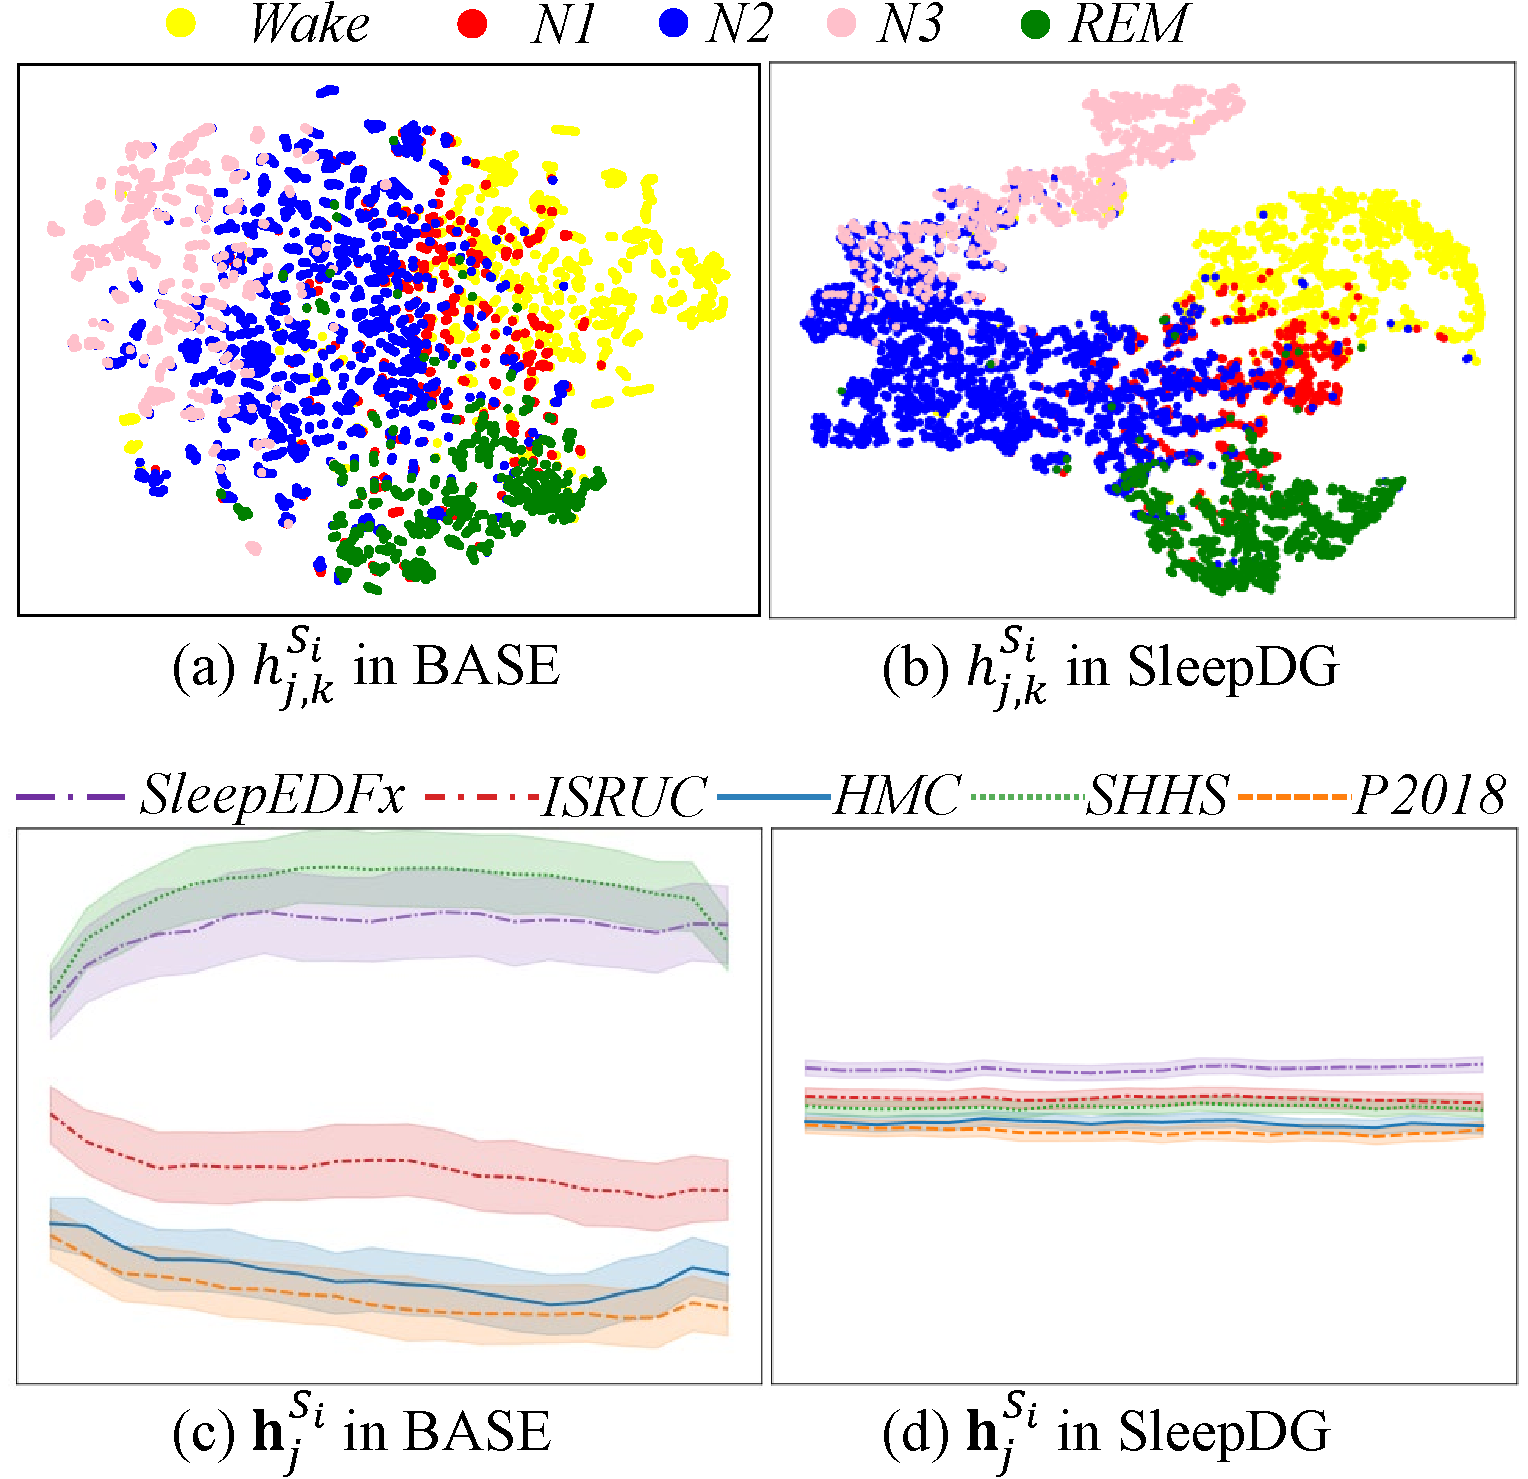
\includegraphics[width=0.99\textwidth]{plt/case.pdf}
    \caption{Examples of a successful case (left) and a failing case (right). In the first case, the person is touching things throughout the video, so the \texttt{ExistsFrame} module returns a uniform distribution on all the frames. The last 2 things the person touches are phone and tissue, though \texttt{Filter} module only finds one correct answer ``phone'', but as it is not equal to the choice ``table'', so \texttt{Equals} module returns the correct final answer ``No''. In the second case, \texttt{Localize} module successfully finds when the person is taking some clothes and \texttt{ExistsFrame} module successfully finds when the person is on the side of something, but \texttt{Filter} module fails to recognize the exact thing that is on the side of the person (probably due to low video quality and the pillow is blocked by the body). Outputs of \texttt{FilterFrame} modules are too complex to be visualized.}
    \label{fig:case}
\end{figure*}

\end{document}